
\documentclass[11pt]{amsbook}

\usepackage{../HBSuerDemir}	% ------------------------

\begin{document}

%++++++++++++++++++++++
\hPage{b1p1/009}
%++++++++++++++++++++++
	The positive square root of $a(>0)$ is denoted by $\sqrt a $ and the negative one by $-\sqrt a$. Thus, \par

	\medskip

	{\centering $\sqrt 4 = 2, \quad -\sqrt4 = -2, \quad \sqrt{(-3)^2} = \sqrt9 = 3$  \\} 

	\medskip 
	
	The number $0$ which is neither positive nor negative has only one square root, namely $0$, as a double root of $x^2 = 0$.  \\ \par

	\underline{ Absolute value \\} 
	
	The \underline {absolute value} of a real number "a" is a non negative real number, denoted by $|a|$ and defined by \\ \par
	
	\medskip
	
	{\centering $ |a| = \sqrt a^2 \quad (\geq 0)$  \\}

	\medskip
	
	or equivalently, by \\
	
	\medskip

	{\centering $ |a| = $  $\begin{cases}

		a \quad if \quad a>0  \\

		0 \quad if \quad a=0 \\

		-a \quad if \quad a<0 \\

	\end{cases}  $\\}

	\medskip
	
	The equivalency of two definitions can be seen by considering three cases $a>0, a=0, a<0$ seperately.

	\medskip

	$ |5| = \sqrt {5^2} = 5, \quad \quad \quad \quad |-3| = \sqrt{(-3)^2} = \sqrt 9 = 3 $ \\

	$ |-2| = -(-2) = 2, \quad \enskip |2| = 2$ \\

	As an immediate corollary we have

	 \medskip

	\underline{Corollary}
	
	\medskip
	
	1. $|a|^2 = a^2 \quad \quad \quad \quad \quad 2. -|a| \leq a \leq |a| $
	
	\medskip

	Some other properties are stated in the next theorem. \\

	\underline{Theorem.} If a, b are real numbers, then 

% ++++++++++++++++++++++++++++++++++++++
\hPage{b1p1/15}
% ++++++++++++++++++++++++++++++++++++++
will be treated in Chapter.\\

We conclude this secftion by two classification of numbers:\\\\

%\begin{figure}[htb]
%	\centering
	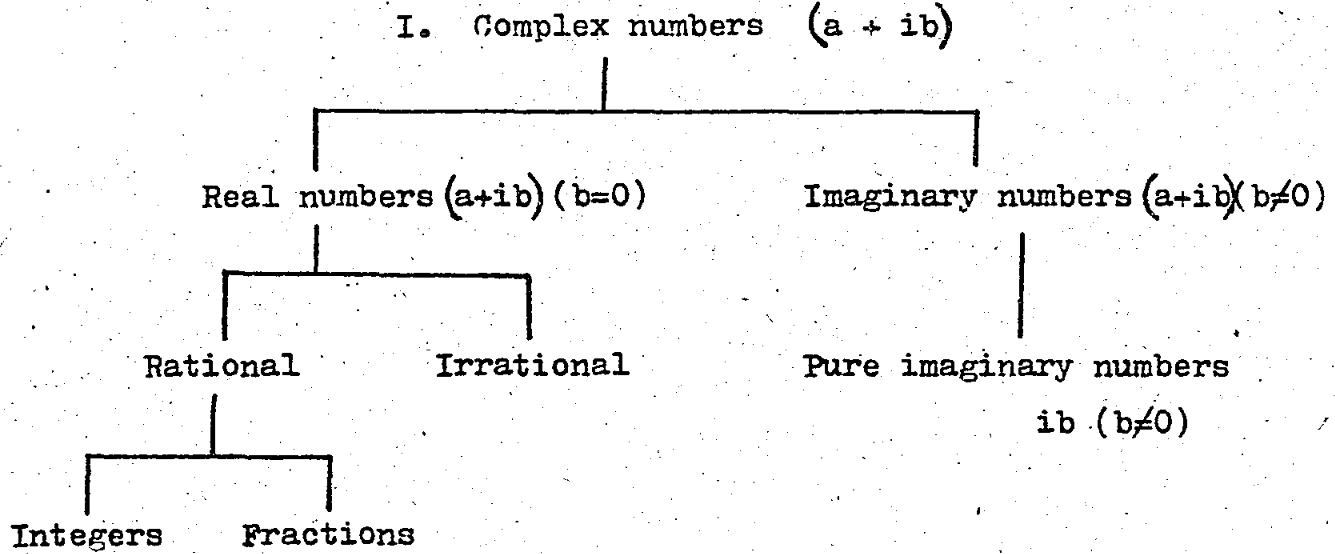
\includegraphics[width=1\textwidth]{images/b1p1-015-fig01}
%	\caption{Classification of complex numbers}
%	\label{fig:classificationOfComplexNumbersA}
%\end{figure}

%\begin{figure}[htb]
%	\centering
	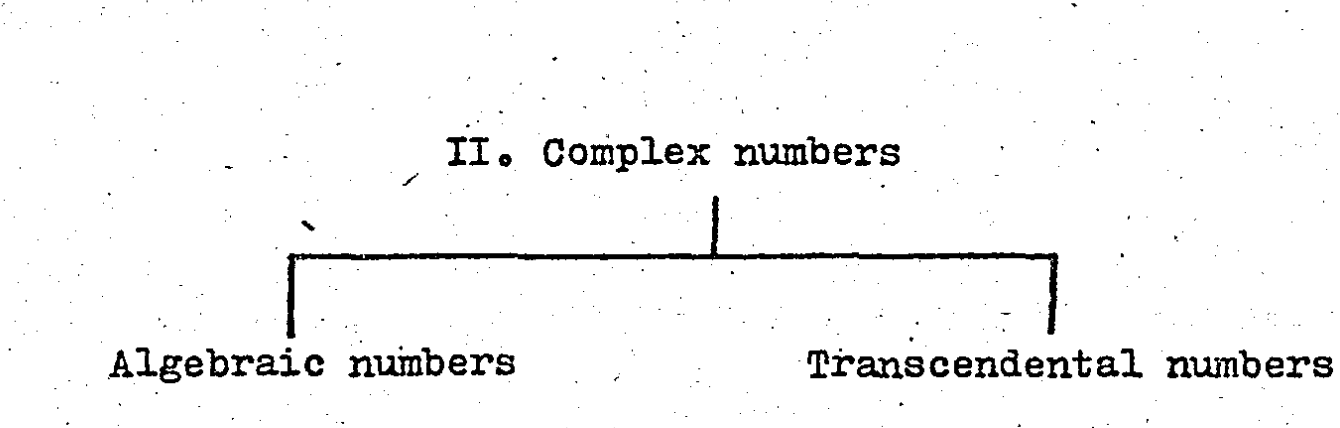
\includegraphics[width=1\textwidth]{images/b1p1-015-fig02}\\
%	\caption{Classification of complex numbers}
%	\label{fig:classificationOfComplexNumbersA}
%\end{figure}

\subsection{EXERCISES}
\paragraph{}

\paragraph{\hspace{0.5cm}1. Construct the following numbers on the number axis:}

\paragraph{\hspace{1.5cm}a) $3/5$\hspace{2.6cm}	b) $-7/3$\hspace{0.6cm} \emph{(use Thales Theorem)}}

\paragraph{\hspace{1.5cm}c) $\sqrt{8}$\hspace{2.8cm}	d) $\sqrt{12}$ \hspace{0.8cm}\emph{(use Pythagorean Theorem)}}

\paragraph{}
\paragraph{\hspace{0.5cm}2. Give examples of two irrational numbers such that their}


% ++++++++++++++++++++++++++++++++++++++
\hPage{b1p1/19}
% ++++++++++++++++++++++++++++++++++++++

The meanings of the symbols
$ \{ x: p(x) \text{ and } q(x) \} $
and
$ \{x: p(x) \text{ or } q(x)\} $
are clear.

\begin{exmp} 
	(for finite sets):
	
	\begin{hEnumerateArabic}	 
		\item
		$ D = \{ n: n \text{ is a digit} \} = \{ 0, 1, 2, \dotsc, 9 \} $
	 
		\item
		$ \{ n: n \in D, n \text{ is prime} \} = \{ 2, 3, 5, 7 \} $
	 
		\item
		$ \{ n: n \in D, 1 \leq n < 7 \} = \{ 1, 2, 3, 4, 5, 6 \} $	 
	\end{hEnumerateArabic} 
\end{exmp}


\begin{exmp} 
	The following infinite sets of numbers are used frequently in mathematics:
	
	\begin{hEnumerateArabic}	 
		\item
		$ \hSoN = \{ n : n \text{ is a natural number} \} = \{ 1, 2, \dotsc, n, \dotsc \} $
		
		\item
		$ \hSoZ = \{ n : n \text{ is an integer} \} = \{ \dotsc, -2, -1, 0, 1, 2, \dotsc \} $
		
		\item
		$ \hSoQ = \{ r : r \text{ is a rational number} \} = \{ \frac{p}{q} : p, q \in \hSoZ, q \neq 0 \} $
		
		\item
		$ \hSoQ'= \{ r' : r' \text{ is an irrational number} \} $

		\item
		$ \hSoR = \{ x : x \text{ is a real number} \} = \{ x : x \in \hSoQ \text{ or } x \in \hSoQ' \} $
		
		\item
		$ \hSoC = \{ z : z \text{ is a complex number} \} = \{ a + ib : a, b \in \hSoR, i^{2} = -1 \} $	 
	\end{hEnumerateArabic} 
\end{exmp}


A set worth of mentioning is the one having no element at all. 
It is called the \hDefined{empty set} (\hDefined{null set}) and denoted by
$ \emptyset $,
so that
$ n(\emptyset) = 0 $.


\begin{exmp} 
	Each one of the following is the null set
	$ \emptyset $:
	
	\begin{hEnumerateArabic}	
		\item
		$ \{ x : x^{2} + 1 = 0 , x \in \hSoR \} $

		\item
		$ \{ x : \hAbs{x} < 0 , x \in \hSoR \} $

		\item
		$ \{ x : x \text{ is a box, } x \text{ is open and } x \text{ is closed} \} $
	\end{hEnumerateArabic} 
\end{exmp}


In any particular discussion, a set that contains all the objects that enter into that discussion is called the \hDefined{uni-}

% ++++++++++++++++++++++++++++++++++++++
\hPage{b1p1/53}
% ++++++++++++++++++++++++++++++++++++++


function given by the rule $ y = \hAbs{x-1} - 2\hAbs{x}+ x $ to be \\
a) a constant function, \\
b) an invertible function.

\begin{hSolution}
	The given function is the piecewisely defined function:
	\[
		y = 
		\begin{cases}
			1+2x & \text{if }x \in(-\infty, 0] \\
			1-2x & \text{if }x \in(0, 1] \\
			-1 & \text{if }x \in(1, \infty).
		\end{cases}
	\]
\footnote{Corrected: "0)" in the first case of the equation must be closed interval "0]"}
\footnote{Corrected: Missing element of sign in the third case}
\end{hSolution}\\
% There must be    \end{exmp}     because the example and its solution is 
%divided into two pages and i could not write it without \begin{exmp} 
%which must be in the previous page.
a) A domain of restriction is $(1, \infty)$, \\
b) A domain of restriction is $(-\infty, 0]$ on which the function is increasing, or (0, 1] on which it is decreasing.

% =======================================
\subsection{Operation with functions}
Let
\[
	f\colon I \to \hSoR,\quad y = f(x)
\]
be a function with domain I. If $c \in \hSoR$, then the function
\begin{align}
	\label{eq:b1p1_053_scalarMultiple}
	cf\colon I \to \hSoR,\quad y = (cf)(x) = cf(x)
\end{align}
is called a \hDefined{scalar multiple} of f.

Let now be given two functions
\begin{gather*}
	f\colon I \to \hSoR,\quad y= f(x) \\
	g\colon J \to \hSoR,\quad y= g(x)
\end{gather*}
with non disjoint domain I and J, then f+g, f-g, fg,

% ++++++++++++++++++++++++++++++++++++++
\hPage{b1p1/17}
% ++++++++++++++++++++++++++++++++++++++

10. Find the distance between the given points. First express them as absolute value, and then compute.
    
    a) 2,72 and 5,16 \qquad b) 3,86 and -7,28
    
	c) -3,86 and 7,28\qquad d) -1,23 and -12,35
    
    11. $(i+3)^3$=? \qquad Ans.\qquad18+26i
    
    12. $\frac{2+i}{3-2i}=? \qquad Ans.\qquad \frac{4+7i}{13}$
    
    13. Write a polynomial of least degree with real coefficients having the roots 3, 1-2i.[$x^3-5x^2+11x-15$]
    
    14. Solve for real X and y :
    \begin{center}
	$\frac{2-i}{3+iy}=\frac{2x-3iy}{2+i}$\qquad Ans.\qquad x=5/6, y=0
	\end{center}
    15. If z=5+4i find $z^2-2z+z\bar{z}$\qquad Ans.\qquad 60+32i
	
    \subsection{SETS}
    \subsubsection{Definitions}
    \qquad Any collection of objects (concrete or abstract) is called a \underline{set}, and the objects in the set are its \underline{elements} or \underline{members}.
    
    \qquad The sets are usually represented by capital letters A, B, ... . Two sets formed by the same elements are said to be \underline{equal}.
    
    \qquad The set A consisting of elements, say, 2, a, Ankara, -7, is denoted either by listing the elements within two braces, or by a diagram (Venn diagram) in which the elements
% ++++++++++++++++++++++++++++++++++++++
\hPage{b1p1/21}

$$A\subseteq B \ and \ B\subseteq A  \ \Longleftrightarrow \ A=B$$

\par \ \par This implication can be used to prove equality of sets.

Some subsets of R are in so frequent use that they bear special symbols, namely:

$$R^+=\{x: \ x>0,x\in R \}, \ R^-=\{x: \ x<0,x\in R \}, \ R^*=\{x: \ x\in R,x\neq 0 \}$$

In the same way we may talk about the subsets of $\mathbb{Q}$, $\mathbb{Z}$ and $\mathbb{N}$ (Why $\mathbb{N}^-=\emptyset$ ? However some authors use $\mathbb{N}^-$ for $\mathbb{Z}^-$. In our notation, $\mathbb{N}^-$ is the set of all negative elements of $\mathbb{N}$, which is the empty set.)

\begin{enumerate}
  \item[C.] \underline{Operations with sets}
\end{enumerate}

Given two sets A and B, by means of three operations "$\cap$", "$\cup$" and "$\setminus$" we define the three sets, namely

\begin{enumerate}
  \item $A\cap B=\{ x: x\in A \ and \ x\in B\}$  "A intersection B"
  \item $A\cup B=\{ x: x\in A \ or \ x\in B\}$  "A union B"
  \item $A\setminus B=\{ x: x\in A,\ x\not \in B\}$  "A minus B"
\end{enumerate}

Venn diagrams of these sets are indicated by shaded sets given below:

\par \ 

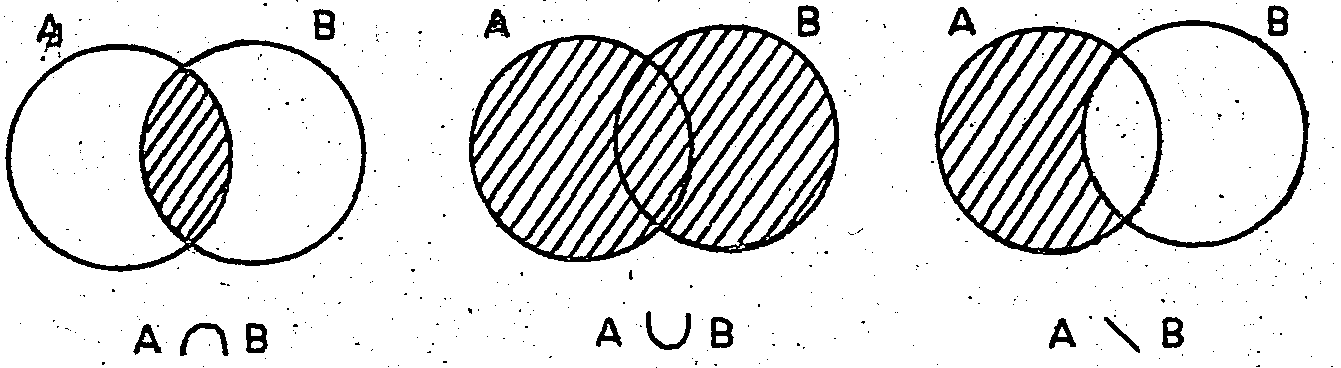
\includegraphics[scale=0.3]{images/b1p1-021-fig01}
% ++++++++++++++++++++++++++++++++++++++
\hPage{b1p1/055}
% ++++++++++++++++++++++++++++++++++++++
\begin{exmp}
	\footnote{example enumeration continues from the previous page.}
	\begin{enumerate}
		\item condition is jointly written with the rule.
		\item \begin{align*}
			(\frac{f}{g})(x) = \frac{f(x)}{g(x)} = \frac{\hAbs{x}}{x^{2}\sqrt{1-x}}
		\end{align*}
		As to the composition $g \circ f$ and $f \circ g$ we have.
		\item \footnote{g(f(x) written for the first equation here in the original book, so I corrected them.}
		\begin{align*}
			(g \circ f)(x) = g(f(x)) &= g(\frac{\hAbs{x}}{x}) = \frac{\hAbs{x}}{x}\sqrt{1-\frac{\hAbs{x}}{x}} \\
			(f \circ g)(x) = f(g(x)) &= f(x\sqrt{1-x}) = \frac{\hAbs{x\sqrt{1-x}}}{x\sqrt{1-x}} = \frac{\hAbs{x}\sqrt{1-x}}{x\sqrt{1-x}} \\
			&= \frac{\hAbs{x}}{x} \quad (x \neq 1)
		\end{align*}
		and \begin{align*}
			D_{g \circ f} = (-\infty, 1] - \hPairingCurly{0}, \: D_{f \circ g} &= (-\infty, 1] - \hPairingCurly{0,1} \\
			&= (-\infty, 1) - \hPairingCurly{0} = (-\infty, 1)
		\end{align*}
	\end{enumerate}
\end{exmp}

\begin{exmp}
	Given the functions
	\begin{align*}
		\hFunction{f}{\hSoR}{\hSoR}, \quad f(x) = \frac{x}{x-2}; \quad \hFunction{g}{\hSoR}{\hSoR}, \quad g(x) = x^{2}-x
	\end{align*}
	find the rules for the composite functions $g \circ f$ and $f \circ g$, and then determine their domains.
	\begin{hSolution}
		\begin{align*}
			1.\: (g \circ f)(x) &= g(f(x)) = f^{2}(x)-f(x) = \frac{x^{2}}{(x-2)^{2}} - \frac{x}{x-2} \\
			&= \frac{x^{2}-x(x-2)}{(x-2)^{2}} = \frac{2x}{(x-2)^{2}} \\
		\end{align*}
		\begin{align*}
			2.\: (f \circ g)(x) = f(g(x)) = \frac{g(x)}{g(x)-2} = \frac{x(x-1)}{(x+1)(x-2)}
		\end{align*}
		\begin{align*}
			D_{g \circ f} = \hSoR - \hPairingCurly{2}, \qquad D_{f \circ g} = \hSoR - \hPairingCurly{-1, 2}
		\end{align*}
	\end{hSolution}
\end{exmp}
% ++++++++++++++++++++++++++++++++++++++
\hPage{b1p1/53}
% ++++++++++++++++++++++++++++++++++++++


function given by the rule $ y = \hAbs{x-1} - 2\hAbs{x}+ x $ to be \\
a) a constant function, \\
b) an invertible function.

\begin{hSolution}
	The given function is the piecewisely defined function:
	\[
		y = 
		\begin{cases}
			1+2x & \text{if }x \in(-\infty, 0] \\
			1-2x & \text{if }x \in(0, 1] \\
			-1 & \text{if }x \in(1, \infty).
		\end{cases}
	\]
\footnote{Corrected: "0)" in the first case of the equation must be closed interval "0]"}
\footnote{Corrected: Missing element of sign in the third case}
\end{hSolution}\\
% There must be    \end{exmp}     because the example and its solution is 
%divided into two pages and i could not write it without \begin{exmp} 
%which must be in the previous page.
a) A domain of restriction is $(1, \infty)$, \\
b) A domain of restriction is $(-\infty, 0]$ on which the function is increasing, or (0, 1] on which it is decreasing.

% =======================================
\subsection{Operation with functions}
Let
\[
	f\colon I \to \hSoR,\quad y = f(x)
\]
be a function with domain I. If $c \in \hSoR$, then the function
\begin{align}
	\label{eq:b1p1_053_scalarMultiple}
	cf\colon I \to \hSoR,\quad y = (cf)(x) = cf(x)
\end{align}
is called a \hDefined{scalar multiple} of f.

Let now be given two functions
\begin{gather*}
	f\colon I \to \hSoR,\quad y= f(x) \\
	g\colon J \to \hSoR,\quad y= g(x)
\end{gather*}
with non disjoint domain I and J, then f+g, f-g, fg,


% ++++++++++++++++++++++++++++++++++++++
\hPage{b1p1/124}
% ++++++++++++++++++++++++++++++++++++++


% =====================================

\begin{thm} \footnote{The theorem and the proof starts in the previous page. 
                                      Begin tags should be removed.}

	\begin{proof}
		exists at $ x_0$ and it is the slope of the 
		\hDefined{unique} 
		tangent line at $x_0$. Consequently, if $f(x)$ has derivative at $x_0$, 
		(then the curve represented by this function has (unique) tangent line with slope $f^\prime(x_0)$, 
                     and normal line with slope $-1/f^\prime(x_0)$. 
		Then we have the equations of tangent and the normal lines through $(x_0,f(x_0))$ with known slope:
		\[
			y - f(x_0) = 
					f^\prime(x_0) 
						\cdot 
							(x-x_0)
		\]
		and
		\[
			y - f(x_0) = 
					- \frac
						{1}
						{f^\prime(x_0)} 
							\cdot 
								(x-x_0)
		\]
	\end{proof}

\end{thm}

% =====================================

The slope of the tangent line at a point is the 
\hDefined{slope of the curve} 
$y = f(x)$ at the same point. Let $\alpha$ be the angle between the positive $x$-axis and the tangent line at $x_0$. 
Then $\tan \alpha = f^\prime(x_0)$ where $\alpha = \arctan f^\prime(x_0)$ is the 
\hDefined{slope angle} 
of the curves at $x_0$.\\

% =====================================

The \hDefined{angle between two curves} 
at a certain common point is defined to be the angle between the tangent lines at this point.
Two curves intersect each other 
\hDefined{orthogonally}
at a point if the angle between them is $90^{\circ}$ at that point, 
and they are tangent at $x_0$ if the angle of intersection is zero at $x_0$.\\

% =====================================

\begin{exmp}

	Find the equations of tangent and normal lines at the points of intersects of the following curves of
	$y = f(x) = x^2$,\\
	$y = g(x) = \sqrt{8x}$, 
	and the angles between their point of intersection.

	\begin{hSolution}
		Equating $y$'s we have $x^4 = 8x 
		\Rightarrow x_1 = 0$, $x_2 = 2 
		\Rightarrow y_1 = 0$, $y_2 = 4$ 
		and the points of intersection are $O = (0,0)$, $A = (2,4)$.
	\end{hSolution}

\end{exmp}


  \hPage{b1p1/225}
    \begin{hEnumerateArabic}
    
        \setcounter{enumi}{180}
        \item {Find $m$, $M$ of the function $f(x) = ( {x} / {x+1} )$} 
        
        \item{Same question for $f(x) = \sqrt[3]{ {x} / ({x^2+1})}$}
        
        \item{Same question for $f(x) = \sin({x}) + \sqrt{3} \cos({x})$}
        
        
        \item{If $m$, $n$ are positive integers with $m > n$, prove. }
        
            \begin{hEnumerateAlpha}
                \item $\frac{x^m - 1}{m} > \frac{x^n - 1}{n}$ , for $x > 1$
                \item $\frac{x^m - 1}{m} > \frac{x^n - 1}{n}$ , for $0 < x < 1$
            \end{hEnumerateAlpha}
        
        \item{Prove the inequalities is Exercise 184 for $m$, $n\in Q$ .}
        \item{If $f(x) = x + 2$ and $g(f(x)) = x^2 - 3x$, find $g(x)$. }
        \item{Defining }
        
        \[
            \max{\{ f(x), g(x) \}} =\begin{cases}
                                        f(x) \text { when } f(x) \ge g(x)\\
                                        g(x) \text { when } g(x) \ge f(x),
                                    \end{cases}
        \]
        
        \[
            \min{\{ f(x), g(x) \}} =\begin{cases}
                                        f(x) \text { when } f(x) \le g(x)\\
                                        g(x) \text { when } g(x) \le f(x),
                                    \end{cases}
        \]
        
        \noindent
        prove that if $f(x), g(x)$ are continuous, then 
        
            \begin{hEnumerateAlpha}
                \begin{multicols}{2}
                    \item $\max{\{ f(x), g(x) \}}$
                \columnbreak
                    \item $\min{\{ f(x), g(x) \}}$
                \end{multicols}
            \end{hEnumerateAlpha}

        are continuous.
        
        \item{ Sketch $\max{\{ f(x), g(x) \}}$ where}
        
            \begin{hEnumerateAlpha}
                \begin{multicols}{2}
                    \item $f(x) = x^2 ,$ $ g(x) = x$
                \columnbreak
                    \item $f(x) = 1 ,$ $ g(x) = x^2$
                \end{multicols}

                \begin{multicols}{2}
                    \item $f(x) = x^2 ,$ $ g(x) = x^2 + 1$
                \columnbreak
                    \item $f(x) = x^3 - x ,$ $ g(x) = 2x - 2$
                \end{multicols}
            \end{hEnumerateAlpha}
        
        \item{For the given functions in Exercise 188, sketch $\min{\{ f(x), g(x) \}}$ }
        
        \item{Sketch: }
            \begin{hEnumerateAlpha}
                \begin{multicols}{2}
                    \item $\{(x , y) : max{\{x,y\}} = 2\}$
                \columnbreak
                    \item $\{(x , y) : min{\{x,y\}} = 2\}$
                \end{multicols}
            \end{hEnumerateAlpha}
        
    \end{hEnumerateArabic}
%%%%%%%%%%%%%%%
\hPage{b1p1/232}
%%%%%%%%%%%%%%%%%%5
\begin{hEnumerateArabic}
    \setcounter{enumi}{207}
    \item  
        \begin{hEnumerateAlpha}
            \begin{multicols}{2}
                \item 1,
                \columnbreak
                \item -1
            \end{multicols}
        \end{hEnumerateAlpha}
    \setcounter{enumi}{209}
    \item $ r = (r_1 + \ldots + r_n ) / n. $
\end{hEnumerateArabic}
\end{document}  

